\documentclass[letterpaper,10pt]{article}
\usepackage[T1]{fontenc}
\usepackage[utf8]{inputenc}
\usepackage{lmodern}
\usepackage{amsmath}
\usepackage{cancel}
\usepackage[margin=1.5in]{geometry}
\usepackage{verbatim}
\usepackage{scrextend}
\usepackage{longtable}
\usepackage{framed}
\usepackage{amssymb}
\usepackage{wasysym}
\usepackage{multicol}
\usepackage{graphicx}
\usepackage{color}
\usepackage{caption}
\usepackage{subcaption}
\usepackage{float}
\usepackage{fancyhdr}
\usepackage[utf8]{inputenc}
\usepackage[mathletters]{ucs}
\usepackage{hyperref}
\usepackage{tikz,tkz-euclide}
\usepackage{pstricks,pst-plot,pst-node,pstricks-add}

\hypersetup
{
  colorlinks=false,
	pdfborder={0 0 0}
}


\pagestyle{fancy}
\lhead{Joseph Mate - jmate - 20246021}
\rhead{CS 648 - Professor Ilyas - UI Optimizer}
\DeclareRobustCommand\iff{\;\Longleftrightarrow\;}

\begin{document}

\raggedright

\setlength{\columnseprule}{0.5pt}


\section{Introduction}
The Postgres query planner does not necessarily return the best plan even with
interesting orders. As mentioned in the CORDS paper, one reason is the estimated
numbers of rows returned by a scan or join can be way off \cite{Ilyas04}. For
instance, imagine the estimate claiming that 1 row is returned from both
relations in a join. The optimizer might estimate one row because of the
indepedence assumption of AND clauses. The optimizer might do nested loop
because everything fits in memory. \\[0.5cm]

As a result, I've created this prototype to explore the possibility of an
database operator manually manipulating the plan, or changing the estimates of
the number rows returned from a base or joined relation.

\section{Features}
I have implemented a UI that displays the plan that the optimizer initially
computes. The UI can display any number of levels of joins. From that UI, you
can change which join algorithm should be applied on two relations. Lastly, the
UI also allows you to modify the the estimated number of rows for each relation
and then the query planner re-searches for a new plan.

\section{How it Works}
Here I provided a summary of the most complicated components of this project. A
lot of challenges I encountered are not included here to keep the report brief.

\subsection{UI}
The UI was built using GTK+. The most complicated component is the display of
tree. This was solved using a table like GUI abstraction, which a GUI widget can
be placed at any row and column of the table. The follow diagram illustrates how
the formula was derived.

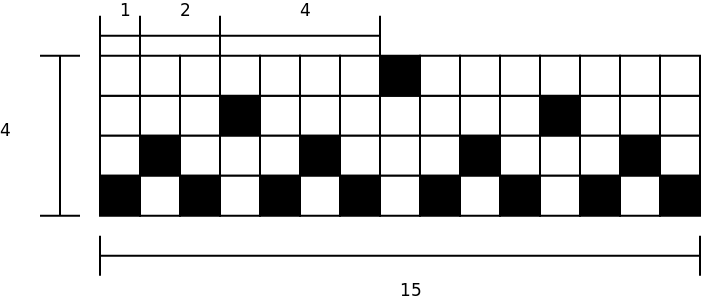
\includegraphics[scale=0.5]{table-derivation.png}

The number of rows is the height of the plan. The child node of a parent, is 1
row below the parent. Additionally, it is $2^{ParentHeight-2}$ units to the left
or the right of the parent.

\subsection{Changing Joins}
We wrap the plan tree datastructure returned by query planner inside our own
tree so that each node of the tree has pointers to any important GUI widgets
that the user may have manipulated. When the user changes the join on the GUI,
we recursively rebuild the path upwards starting from the node that was changed.

\subsection{Changing a Relation's Rows Estimates}
We add a hashtable to the PlannerInfo struct. The hashtable is a map from relids
of the relation to the overridden number of rows. If the hashtable does not
contain an entry for a given relids, then the estimate for that relation has not
been overridden. Where ever the estimated number of rows was accessed in costsize.c, we
prepended a lookup to the hashtable to check if it has been overridden.

\section{Future Plans}
Firstly, this GUI runs on the database process. In order to keep the scope of
the project minimal, I decided to not create somone messaging protocol for
communicating back and forth with the database server. Secondly, currently there
is no way to maniupate the structure of the tree. Thirdly, there is no way to
change which scan should be performed on a based relation. Fourthly, only one
pathkey is considered for the merge join. A variety of options should be
presented to the user selecting merge join. Lastly, there is absolutely no
validation.

\nocite{*}               
\bibliographystyle{plain}
\bibliography{write-up}     


\end{document}
